\documentclass[tikz, border=2mm]{standalone}
\usepackage{tikz}
\usetikzlibrary{patterns.meta} % For advanced patterns

\begin{document}
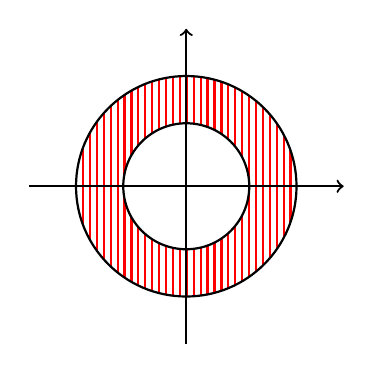
\begin{tikzpicture}

% Define radii
\def\innerRadius{0.8}
\def\outerRadius{1.4}

% --- Draw the Annulus using pre/post actions FIRST ---

% 1. Draw the Outer Circle:
%    - Preaction: Fill the entire outer circle with the pattern.
%    - Main Action: Draw the thick black border of the outer circle.
\path[
    preaction={
        fill, % Specify fill action
        pattern={Lines[angle=90, distance=2.5pt, line width=0.8pt]}, % Define pattern
        pattern color=red % Set pattern color
    },
    draw=black, % Main action: draw the border
    thick % Border thickness
] (0,0) circle (\outerRadius);

% 2. Draw the Inner Circle:
%    - Preaction: Fill the inner circle area with white. This effectively "erases"
%                 the pattern that was drawn over the whole outer circle area before.
%    - Main Action: Draw the thick black border of the inner circle on top of the white fill.
\path[
    preaction={
        fill=white % Fill with background color (usually white)
    },
    draw=black, % Main action: draw the border
    thick % Border thickness
] (0,0) circle (\innerRadius);

% --- End Annulus Drawing ---


% --- Draw Axes LAST so they appear on top of the white fill ---
\draw[thick, ->] (-2, 0) -- (2, 0); % Horizontal axis
\draw[thick, ->] (0, -2) -- (0, 2); % Vertical axis
% --- End Axes ---

\end{tikzpicture}
\end{document}